\chapter{Dedicated Microprocessors}\label{ch:dedicated}

\begin{objectives}
After studying this chapter you will be able to:
\begin{itemize}
  \item describe the von Neumann model of a computer and the layers of abstraction from transistors to processors;
  \item explain what a dedicated microprocessor is and how it divides into a \emph{datapath} and a \emph{control unit};
  \item describe computations at the register-transfer level (RTL);
  \item design a datapath for a given algorithm and write its \emph{control words};
  \item design the control unit as an FSM driven by status signals, including a wait state when needed for timing;
  \item implement a dedicated processor in VHDL in the FSM+D style and in the FSMD style.
\end{itemize}
\end{objectives}

\section{The Von Neumann Model}\label{sec:vonneumann}
Almost every computer follows the model described by John von Neumann in 1945~\cite{vonneumann1945}. It has five components (\cref{fig:vn}): \textbf{input} supplies data, \textbf{output} presents results, \textbf{memory} stores programs and data, and the \textbf{microprocessor} (the ``brain'') processes the data. The microprocessor has a \textbf{datapath}, which carries out the data processing (arithmetic and logic), and a \textbf{control unit}, which determines the sequence of operations.

\figw{301.8pt}{lect_9_von_neumann_model}{The von Neumann model of a computer.}{fig:vn}

\section{From Transistors to Microprocessors}
Digital systems are so complex that they can only be designed by managing complexity through \emph{layers of abstraction} (\cref{fig:hier}). Transistors combine into logic gates; gates form combinational and sequential circuits; circuits form functional components such as adders and multiplexers (Chapters~4 and~5) and registers and counters (Chapter~7); and components are integrated into a datapath and a control unit, which together form the microprocessor. Each layer hides the details of the layer below it, so a designer can work at the level of components without thinking of transistors. This chapter works at the top two layers.

\figw{243.9pt}{lect_9_digital_hierarchy}{Layers of abstraction: from transistors to microprocessors.}{fig:hier}

\section{Dedicated Microprocessors}
A \term{dedicated microprocessor} (special-purpose processor) is designed to perform one specific task. The ``program'' is not stored in memory but is \emph{hardwired} in the structure of the processor, which makes it optimised for the task in speed, power and size. Its function cannot be changed after manufacture (if implemented as an ASIC; an FPGA implementation can be reconfigured). Examples are the image-processing chip in a digital camera, the controller in a microwave oven and a GCD engine inside a cryptographic circuit. In contrast, a \emph{general-purpose} processor executes arbitrary programs stored in memory and is the subject of \cref{ch:gp}.

\section{Datapath and Control Unit}\label{sec:dpcu}
A microprocessor is partitioned into two cooperating parts (\cref{fig:dpcu}).
\begin{itemize}
  \item The \term{datapath} performs the data processing operations. It contains functional units (ALUs, adders, comparators), registers, counters and multiplexers; this is where the ``number crunching'' happens.
  \item The \term{control unit} determines the \emph{sequence} of datapath operations. In each clock cycle it generates \term{control signals}, which tell the datapath what to do (load this register, select that input), and it receives \term{status signals} from the datapath (the result is zero, $A>B$) which it uses to make decisions. The control unit is an FSM, as studied in \cref{ch:fsm}.
\end{itemize}

\figw{261.1pt}{lect_9_datapath_control}{A dedicated microprocessor: the control unit sends control signals to the datapath and receives status signals from it.}{fig:dpcu}

\section{Register Transfer Level}\label{sec:rtl}
The \term{register-transfer level} (RTL) is the level of abstraction at which a synchronous digital system is described by (1)~the flow of data between registers and (2)~the logical or arithmetic operations performed on the data on the way (\cref{fig:rtl}). At RTL we consider information moving ``in bulk'' from register to register at each clock tick, ignoring the gates and flip-flops that implement it. This is the level of abstraction of VHDL and Verilog, and of the notation $R_1\leftarrow R_2+R_3$ used in this chapter, meaning ``at the next active clock edge, load $R_1$ with the sum of the contents of $R_2$ and $R_3$''.

\figw{298.3pt}{lect_9_rtl_model}{The RTL model: registers, combinational logic between them, and a common clock.}{fig:rtl}

\section{Datapath Design}\label{sec:datapath}
To design a datapath for a single problem, assemble the registers and functional units needed to perform the required operations, then connect them so that every transfer in the algorithm has a path.

\begin{example}{Datapath for $A=B+C$}{dp1}
Registers $B$ and $C$ hold the operands; an adder forms $B+C$; register $A$ stores the result when the control signal $ALoad$ is asserted (\cref{fig:dp-abc}).
\end{example}

\begin{example}{Datapath for $A=A+3$}{dp2}
The output of register $A$ is fed back to one input of an adder; the other input is the constant 3; the sum is loaded back into $A$ (\cref{fig:dp-a3}). The control unit asserts $ALoad$ once for each addition.
\end{example}

\begin{figure}[htbp]
\centering
\begin{subfigure}[b]{313.3pt}\centering
  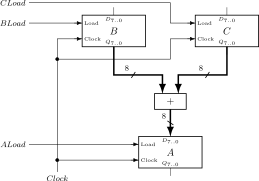
\includegraphics[width=311.3pt]{lect_9_datapath_A_B_plus_C}\caption{$A=B+C$}\label{fig:dp-abc}
\end{subfigure}
\\[6pt]
\begin{subfigure}[b]{198.6pt}\centering
  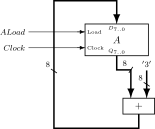
\includegraphics[width=196.6pt]{lect_9_datapath_A_plus_3}\caption{$A=A+3$}\label{fig:dp-a3}
\end{subfigure}
\caption{Two dedicated datapaths.}
\end{figure}

\subsection{Sharing a functional unit with multiplexers}
Suppose the processor must perform \emph{both} $A=A+3$ and $A=B+C$. Two adders would work, but a single adder preceded by multiplexers is cheaper. A multiplexer in front of each adder input selects the operand: the first chooses between $B$ ($0$) and $A$ ($1$), the second between $C$ ($0$) and the constant $3$ ($1$) (\cref{fig:dp-shared}). Because the two operations need either $(B,C)$ or $(A,3)$, one control signal $\mathit{Mux}$ can drive both multiplexers. The control unit selects the operation by the \emph{control word}, i.e.\ the values of all control signals needed in a clock cycle (\cref{tab:cw1}).

\figw{392.6pt}{lect_9_datapath_one_adder}{A shared-adder datapath that performs $A=A+3$ and $A=B+C$. Both multiplexers are driven by the same control signal $Mux$ (input $1$ selects $A$ and the constant $3$, input $0$ selects $B$ and $C$); the bus width is marked with a slash, and the clock is common to all registers.}{fig:dp-shared}

The two multiplexers can also be placed \emph{in front of the destination register} instead: the adder outputs $B+C$ and $A+3$ feed a single 2-to-1 multiplexer $Amux$ that selects what is loaded into $A$ (\cref{fig:dp-combine}). This version needs two adders but only one multiplexer, and the same $ALoad$ and $Amux$ signals again define the two operations.

\figw{265.0pt}{lect_9_datapath_combine}{Alternative datapath for $A=B+C$ and $A=A+3$: one multiplexer $Amux$ in front of register $A$.}{fig:dp-combine}

\begin{table}[htbp]
\centering
\caption{Control words of the shared-adder datapath.}
\label{tab:cw1}
\begin{tabular}{l|cc}
\toprule Operation & $ALoad$ & $Mux$\\ \midrule
$A=A+3$ & 1 & 1\\ $A=B+C$ & 1 & 0\\ \bottomrule
\end{tabular}
\end{table}

\subsection{Status signals and conditional operations}
To implement a conditional such as \textbf{IF} $(A=0)$ the datapath must produce a \emph{status signal} for the control unit. An equality comparator can compare a register with a constant (\cref{fig:dp-if}a). For $A=0$ in an 8-bit register there is a cheaper solution: a single 8-input NOR gate, whose output is 1 only if every bit of $A$ is 0 (\cref{fig:dp-if}b). Similarly, a magnitude comparator (\cref{sec:comparator}) produces $A>B$.

\figw{332.0pt}{lect_9_datapath_if}{Generating the status signal $(A=0)$: (a)~comparator with the constant $0$; (b)~8-input NOR gate.}{fig:dp-if}

\subsection{An if-then-else datapath}
Consider the algorithm
\begin{center}\ttfamily\small
INPUT A;\quad IF (A = 5) THEN B = 8 ELSE B = 13; \quad OUTPUT B
\end{center}
The datapath of \cref{fig:ite-dp} has register $A$ (the input), register $B$ (the result), a multiplexer selecting the constant 8 or 13, an AND gate that generates the status signal $(A=5)$ by decoding the bit pattern $0101$ (the inputs for $A_3$ and $A_1$ are inverted), and an output buffer controlled by $Out$. The control signals are $ALoad$, $BLoad$, $Muxsel$ ($1$ selects 8, $0$ selects 13) and $Out$. The algorithm is converted into a sequence of control words (\cref{tab:cw-ite}); the control unit decides between control words 2 and 3 using the status signal $(A=5)$.

\figw{282.1pt}{lect_9_datapath_if_then_else}{Datapath for the if-then-else algorithm.}{fig:ite-dp}

\begin{table}[htbp]
\centering
\caption{Control words for the if-then-else algorithm.}
\label{tab:cw-ite}
\begin{tabular}{cl|cccc}
\toprule CW & Instruction & $ALoad$ & $Muxsel$ & $BLoad$ & $Out$\\ \midrule
1 & INPUT A & 1 & X & 0 & 0\\ 2 & $B=8$ & 0 & 1 & 1 & 0\\ 3 & $B=13$ & 0 & 0 & 1 & 0\\ 4 & OUTPUT B & 0 & X & 0 & 1\\ \bottomrule
\end{tabular}
\end{table}

\subsection{A datapath with a loop: summing the numbers 1 to 10}
\begin{center}\ttfamily\small
\begin{tabular}{@{}l@{}}
Sum = 0\\ i = 1\\ DO \{\\ \quad Sum = Sum + i\\ \quad i = i + 1\\ \} WHILE (i != 11)\\ OUTPUT Sum
\end{tabular}
\end{center}
The datapath needs two registers, $Sum$ and $i$, an adder, and a gate that signals when $i\neq11$. We build it (\cref{fig:sum-dp}) with \emph{one} adder, whose first input is always $i$ and whose second input is chosen by $\mathit{addMux}$: $Sum$ (0) or the constant 1 (1). The adder output $R$ goes to both registers through input multiplexers: $\mathit{sumMux}$ chooses between $R$ (0) and the constant 0 (1), and $\mathit{iMux}$ between $R$ (0) and the constant 1 (1). With these selections each instruction of the algorithm is one control word (\cref{tab:cw-sum}): $Sum=0$ is $sumLoad=1$, $sumMux=1$; $i=1$ is $iLoad=1$, $iMux=1$; $Sum=Sum+i$ is $sumLoad=1$, $sumMux=0$, $addMux=0$; $i=i+1$ is $iLoad=1$, $iMux=0$, $addMux=1$; and the output is $OE=1$. The loop is made by the control unit (\cref{sec:cu-design}).

\figw{370.5pt}{lect_9_datapath_sum_1_to_10}{A datapath for summing the numbers from 1 to 10 with one adder and three multiplexers. The status signal $(i\neq11)$ is a NAND gate whose inputs for the zero bits of $11=00001011_2$ are inverted; the output $Sum$ is enabled by $OE$.}{fig:sum-dp}

\begin{table}[htbp]
\centering
\caption{Control words for the summation algorithm.}
\label{tab:cw-sum}
\begin{tabular}{cl|cccccc}
\toprule CW & Instruction & $sumLoad$ & $sumMux$ & $iLoad$ & $iMux$ & $addMux$ & $OE$\\ \midrule
1 & $Sum=0$ & 1 & 1 & 0 & X & X & 0\\
2 & $i=1$ & 0 & X & 1 & 1 & X & 0\\
3 & $Sum=Sum+i$ & 1 & 0 & 0 & X & 0 & 0\\
4 & $i=i+1$ & 0 & X & 1 & 0 & 1 & 0\\
5 & OUTPUT $Sum$ & 0 & X & 0 & X & X & 1\\ \bottomrule
\end{tabular}
\end{table}

\section{Control Unit Design}\label{sec:cu-design}
The control unit is an FSM (\cref{fig:dpcu}) that steps through the control words of the algorithm and branches on the status signals. In a Moore machine, each state outputs one control word. We design three control units.

\subsection{Example 1: counting from 1 to 10}
\begin{example}{Counter control unit}{cu1}
The algorithm is \texttt{i = 0; WHILE (i != 10) \{ i = i + 1 \}}. The datapath is a counter $i$ with a clear input and a count input and a comparator producing the status signal $(i=10)$ (\cref{fig:cnt-dp}). The control signals are \emph{Clear} and \emph{Count}.

\textbf{State diagram} (\cref{fig:cnt-fsm}). $S_0$: clear the counter. $S_1$: increment; remain in $S_1$ while $i\neq10$ and leave when $i=10$. $S_2$: the loop is finished. A fourth state $S_3$ (halt) keeps the machine idle after the computation. With the state assignment $S_0=00$, $S_1=01$, $S_2=10$, $S_3=11$ and $x$ denoting the status signal $(i=10)$, the next-state table (\cref{tab:cu1}) and the Moore output table give
\begin{align*}
 D_1 &= Q_1 + Q_0x, & D_0 &= Q_1 + Q_0' + x',\\
 Clear &= Q_1'Q_0' = \overline{Q_1+Q_0}, & Count &= Q_1'Q_0 .
\end{align*}
The control logic is \cref{fig:cnt-logic}; connected to the datapath it forms the complete dedicated microprocessor of \cref{fig:cnt-comb}.
\end{example}

\begin{table}[htbp]
\centering
\caption{Tables of the counter control unit ($x=(i=10)$).}
\label{tab:cu1}
\begin{tabular}{cc|cc}
\toprule PS $Q_1Q_0$ & Input $x$ & NS $D_1D_0$ & \\ \midrule
00 ($S_0$)&X&01 ($S_1$)&\\ 01 ($S_1$)&0&01 ($S_1$)&\\ 01 ($S_1$)&1&10 ($S_2$)&\\
10 ($S_2$)&X&11 ($S_3$)&\\ 11 ($S_3$)&X&11 ($S_3$)&\\ \bottomrule
\end{tabular}\qquad
\begin{tabular}{c|cc}
\toprule State & Clear & Count\\ \midrule
00 ($S_0$)&1&0\\01 ($S_1$)&0&1\\10 ($S_2$)&0&0\\11 ($S_3$)&0&0\\ \bottomrule
\end{tabular}
\end{table}

\begin{figure}[htbp]
\centering
\begin{subfigure}[b]{174.9pt}\centering
  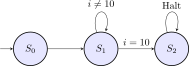
\includegraphics[width=172.9pt]{lect_9_counter_fsm}\caption{control FSM}\label{fig:cnt-fsm}
\end{subfigure}
\hfill
\begin{subfigure}[b]{202.6pt}\centering
  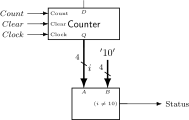
\includegraphics[width=200.6pt]{lect_9_counter_datapath}\caption{datapath}\label{fig:cnt-dp}
\end{subfigure}
\\[6pt]
\begin{subfigure}[b]{300.0pt}\centering
  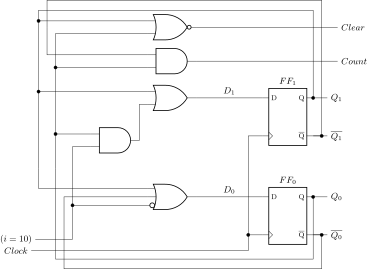
\includegraphics[width=298.0pt]{lect_9_counter_logic}\caption{control logic}\label{fig:cnt-logic}
\end{subfigure}
\caption{The counter processor of \cref{ex:cu1}.}
\end{figure}

\begin{figure}[htbp]
\centering
\ContinuedFloat
\begin{subfigure}[b]{409.4pt}\centering
  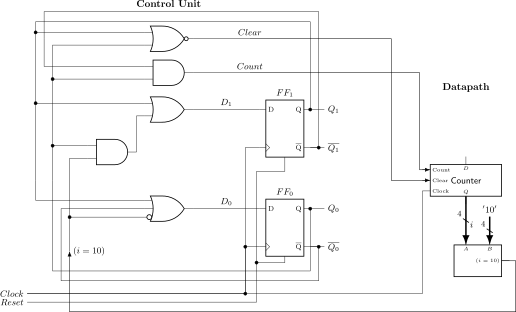
\includegraphics[width=407.4pt]{lect_9_counter_combined}\caption{complete processor}\label{fig:cnt-comb}
\end{subfigure}
\caption[]{The counter processor of \cref{ex:cu1}.}
\end{figure}

\subsection{Example 2: the if-then-else control unit}
\begin{example}{if-then-else control unit}{cu2}
The control signals and control words are those of \cref{tab:cw-ite}; the status signal is $(A=5)$. A first design has the states $S_{input}$ (load $A$), $S_{equal}$ ($B=8$), $S_{notequal}$ ($B=13$) and $S_{output}$, with $S_{input}$ branching directly on the status signal (\cref{fig:ite-fsm-noextra}).

\textbf{The timing problem.} In $S_{input}$ register $A$ is loaded \emph{at the end of the clock cycle}. The control unit takes its branching decision at the same clock edge, so it sees the status signal computed from the \emph{old} contents of $A$ and may go to the wrong state. The simulation of \cref{fig:ite-nowait} shows this error. The remedy is an extra \textbf{wait state} $S_{extra}$ after $S_{input}$, in which nothing happens for one clock period: register $A$ takes its new value and the comparator settles, and the next state is decided in $S_{extra}$ using the correct status (\cref{fig:ite-fsm,fig:ite-wait}).

\textbf{Synthesis.} With the state assignment $S_{input}=000$, $S_{extra}=001$, $S_{notequal}=010$, $S_{equal}=011$, $S_{output}=100$ the next-state table is \cref{tab:ite-ns}. Writing $I$ for the status signal $(A=5)$:
\begin{align*}
 D_2 &= Q_2+Q_1, & D_1 &= Q_1'Q_0, & D_0 &= Q_2'Q_1'(Q_0'+I),\\
 ALoad &= Q_2'Q_1'Q_0', & BLoad &= Q_2'Q_1, & Muxsel &= Q_0, & Out &= Q_2 .
\end{align*}
Muxsel is 1 in $S_{equal}$ (select 8) and 0 in $S_{notequal}$ (select 13); in $S_{extra}$ it is a don't-care. The VHDL is \cref{lst:ite-cu}, in which the state register is built of D flip-flops and the logic is written as the equations above, and \cref{fig:ite-comb} shows the control unit connected to the datapath.
\end{example}

\begin{table}[htbp]
\centering
\caption{Next-state and output tables of the if-then-else control unit with wait state ($I=(A=5)$).}
\label{tab:ite-ns}
\begin{tabular}{cc|c}
\toprule Present state & $I$ & Next state\\ \midrule
000 ($S_{input}$)&X&001\\ 001 ($S_{extra}$)&0&010\\ 001 ($S_{extra}$)&1&011\\
010 ($S_{notequal}$)&X&100\\ 011 ($S_{equal}$)&X&100\\ 100 ($S_{output}$)&X&100\\ \bottomrule
\end{tabular}\qquad
\begin{tabular}{cl|cccc}
\toprule State & Name & $ALoad$ & $Muxsel$ & $BLoad$ & $Out$\\ \midrule
000&$S_{input}$&1&X&0&0\\001&$S_{extra}$&0&X&0&0\\010&$S_{notequal}$&0&0&1&0\\011&$S_{equal}$&0&1&1&0\\100&$S_{output}$&0&X&0&1\\ \bottomrule
\end{tabular}
\end{table}

\begin{figure}[htbp]
\centering
\begin{subfigure}[b]{259.9pt}\centering
  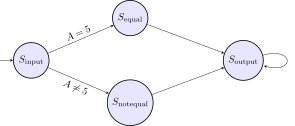
\includegraphics[width=257.9pt]{lect_9_if_then_else_fsm_no_extra}\caption{without wait state}\label{fig:ite-fsm-noextra}
\end{subfigure}
\\[6pt]
\begin{subfigure}[b]{271.2pt}\centering
  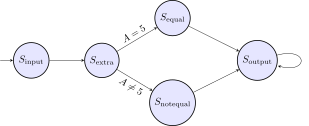
\includegraphics[width=269.2pt]{lect_9_if_then_else_fsm}\caption{with wait state}\label{fig:ite-fsm}
\end{subfigure}
\caption{Control-unit state diagrams for the if-then-else algorithm.}
\end{figure}

\begin{figure}[htbp]
\centering
\wavesplit{lect_9_if_then_else_no_wait}{2}\vspace{3pt}{\small (a)~without wait state: the wrong branch is taken}\\[6pt]
\wavesplit{lect_9_if_then_else_wait_state}{3}\vspace{3pt}{\small (b)~with wait state: the correct branch is taken}
\caption{Simulation waveforms of the if-then-else processor (author's screenshots).}
\label{fig:ite-nowait}\label{fig:ite-wait}
\end{figure}

\vhdlfile{listings/ch09_if_then_else_control.vhd}{Structural VHDL of the if-then-else control unit (state register of D flip-flops and the synthesised equations). The component \code{d_ff_r} is the flip-flop with asynchronous reset of \cref{lst:seqdet-struct}.}{lst:ite-cu}

\figw{410.0pt}{lect_9_if_then_else_combined}{The if-then-else control unit connected to its datapath.}{fig:ite-comb}

\subsection{Example 3: the GCD processor}
\begin{example}{Greatest common divisor}{gcd}
The \emph{greatest common divisor} of two positive integers $X$ and $Y$ can be found by repeated subtraction (Euclid's algorithm): the larger number is replaced by the difference until the two are equal.
\begin{center}\ttfamily\small
\begin{tabular}{@{}l@{}}
INPUT X\\ INPUT Y\\ WHILE (X != Y) \{\\ \quad IF (X > Y) THEN X = X - Y\\ \quad ELSE Y = Y - X\\ \}\\ OUTPUT X
\end{tabular}
\end{center}
For $X=25$, $Y=15$: $X>Y$, so $X=10$; $X<Y$, so $Y=5$; $X>Y$, so $X=5$; now $X=Y=5$, the GCD.

\textbf{Datapath} (\cref{fig:gcd-dp}): registers $X$ and $Y$, each with an input multiplexer that selects the external input or the result of the subtractor, a subtractor whose operands are chosen by multiplexers so that it can compute $X-Y$ or $Y-X$, and comparators that produce the status signals $XeqY$ and $XgtY$. The control signals are \textit{In\_X}, \textit{In\_Y} (select the external input, 1, or the subtractor result, 0), \textit{XLoad}, \textit{YLoad}, \textit{XY} (0: $X-Y$; 1: $Y-X$) and \textit{Out}.

\textbf{Control unit} (\cref{fig:gcd-fsm}). $S_0$ (init): load $X$ and $Y$ from the inputs. $S_1$ (check): compare; go to $S_4$ if $X=Y$, to $S_2$ if $X>Y$, otherwise to $S_3$. $S_2$: $X\leftarrow X-Y$, then back to $S_1$. $S_3$: $Y\leftarrow Y-X$, then back to $S_1$. $S_4$ (done): output the result. \Cref{lst:gcd-cu} is the VHDL of the control unit, with the control signals as Moore outputs. The datapath components and the top-level connection are in \cref{app:listings}, and \cref{fig:gcd-sim} shows the simulation.
\end{example}

\begin{figure}[htbp]
\centering
\begin{subfigure}[b]{412.0pt}\centering
  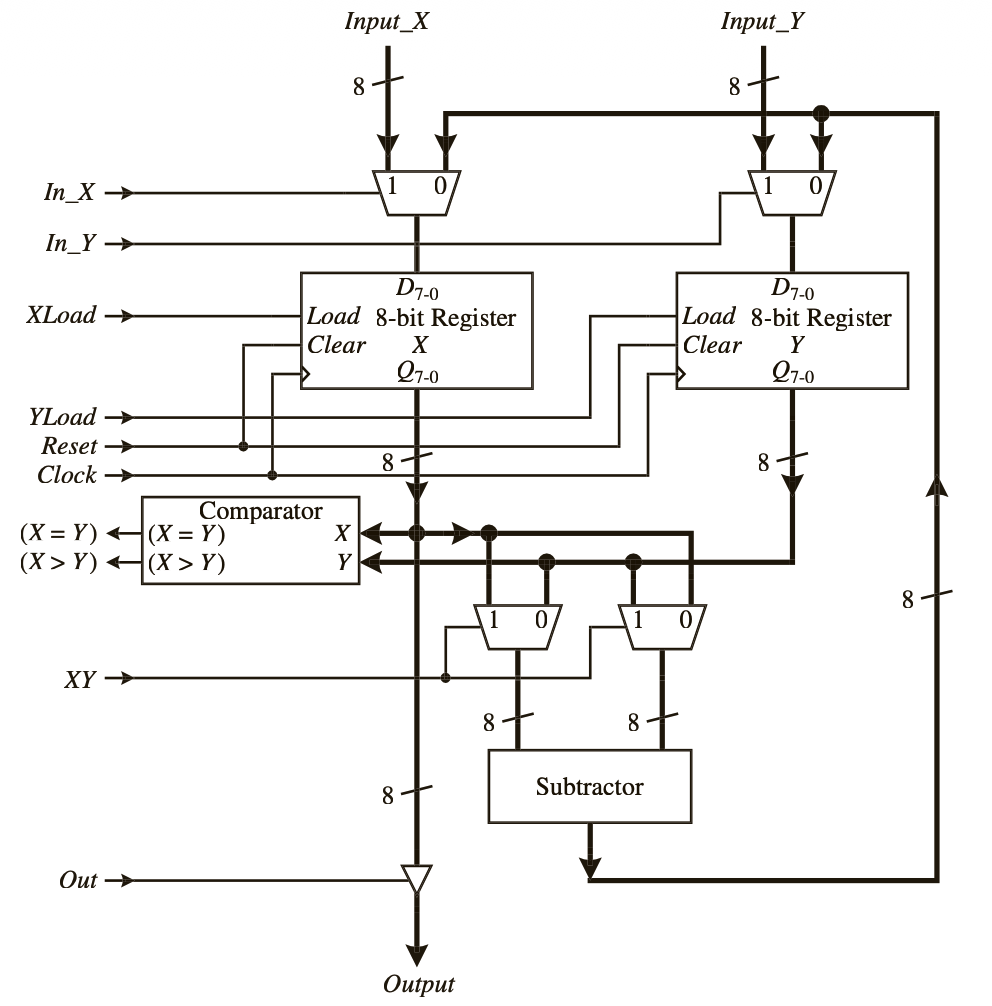
\includegraphics[width=399.0pt]{lect_9_gcd_datapath}\caption{datapath}\label{fig:gcd-dp}
\end{subfigure}
\caption{The GCD processor.}
\end{figure}

\begin{figure}[htbp]
\centering
\ContinuedFloat
\begin{subfigure}[b]{219.0pt}\centering
  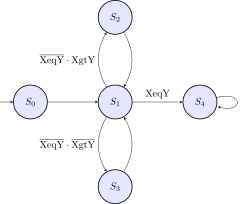
\includegraphics[width=217.0pt]{lect_9_gcd_fsm}\caption{control FSM}\label{fig:gcd-fsm}
\end{subfigure}
\caption[]{The GCD processor.}
\end{figure}

\vhdlfile{../vhdl/gcd/gcd_control.vhd}{VHDL of the GCD control unit (FSM with five states).}{lst:gcd-cu}

\begin{figure}[htbp]
\centering
\wavesplit{lect_9_gcd_sim}{5}
\caption{Simulation of the GCD processor (author's screenshot).}
\label{fig:gcd-sim}
\end{figure}

\section{FSM+D versus FSMD}\label{sec:fsmd}
There are two ways to describe a dedicated processor in an HDL.
\begin{description}[font=\sffamily\bfseries, leftmargin=1.2em]
  \item[FSM+D (FSM plus datapath)] The control unit (FSM) and the datapath are designed as \emph{separate, explicitly constructed} units and connected in a top-level module, as in the examples so far. The designer has full control over the datapath structure, which is useful for highly optimised or unusual datapaths.
  \item[FSMD (FSM with datapath)] The whole design is described as \emph{one behavioural FSM}, with the datapath operations (such as \code{X <= X - Y;}) written inside the states. The synthesis tool infers the registers, adders and multiplexers and connects them to the control logic. This is faster and simpler for standard operations and is the most common modern approach~\cite{gajski1997}.
\end{description}
\Cref{lst:gcd-fsmd} is the GCD calculator as an FSMD. The state diagram is the same as \cref{fig:gcd-fsm}, but each state now contains the register transfer it performs. Compare its length with the FSM+D version; the RTL viewer (\cref{fig:gcd-fsmd-rtl}) shows that the synthesis tool has generated the comparators, subtractors and registers by itself.

\vhdlfile{../vhdl/gcd_fsmd.vhd}{The GCD calculator as an FSMD: datapath operations inside a single behavioural state machine.}{lst:gcd-fsmd}

\begin{figure}[htbp]
\centering
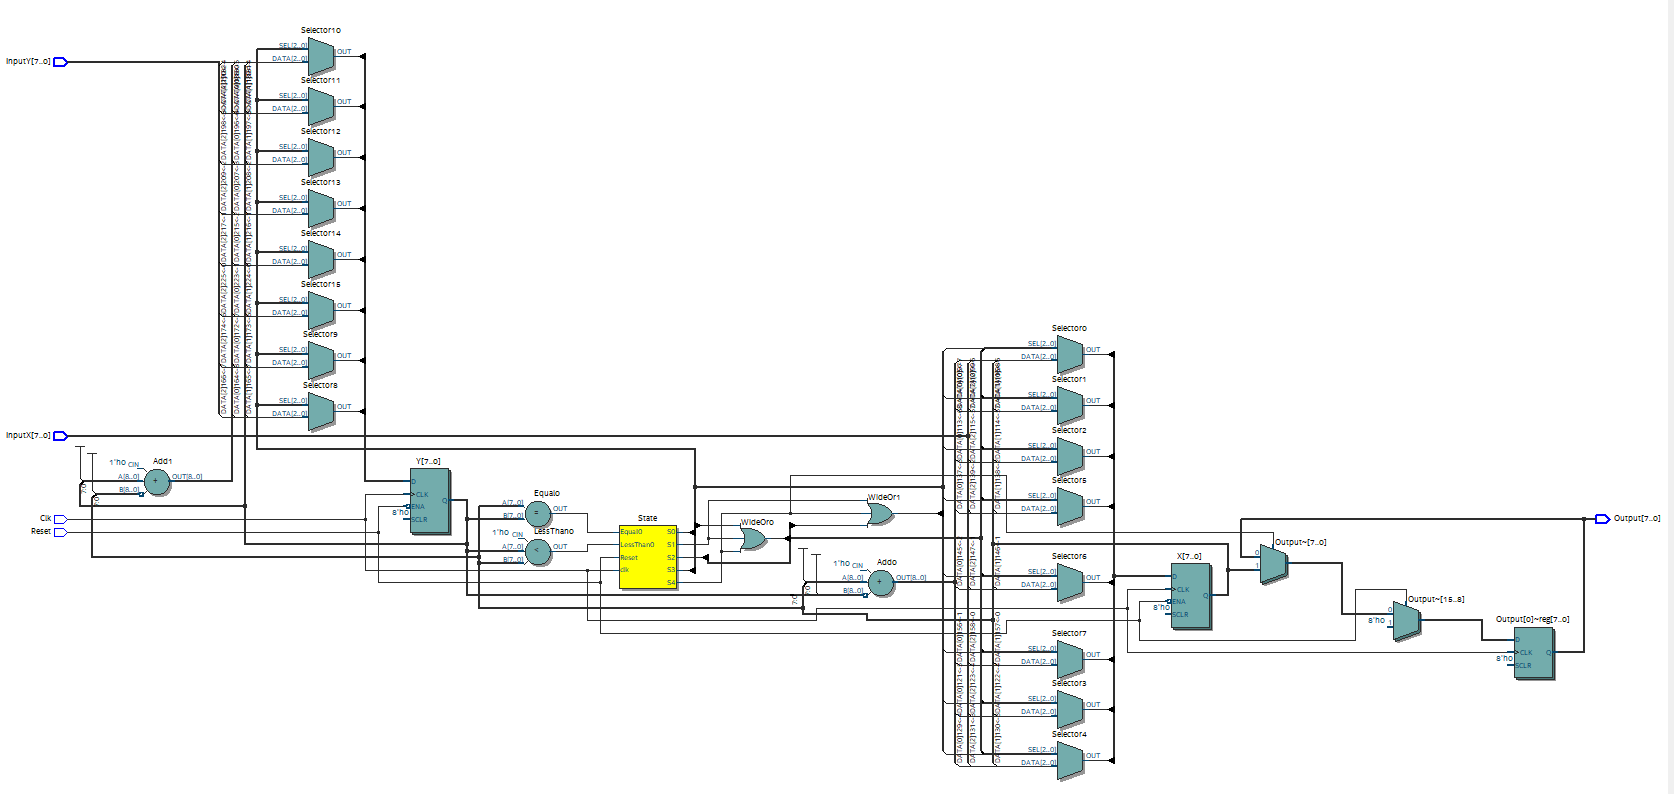
\includegraphics[width=0.9\linewidth]{lect_9_gcd_fsmd}\\[6pt]
\foreach \wsi in {1,...,4}{\includegraphics[width=\linewidth,height=95pt,keepaspectratio]{lect_9_gcd_fsmd_sim_p\wsi}\par\vspace{1.5pt}}
\caption{The FSMD GCD: logic diagram from the Quartus RTL viewer (top) and simulation (bottom). Author's screenshots.}
\label{fig:gcd-fsmd-rtl}
\end{figure}

\begin{chaptersummary}
\begin{itemize}
  \item The \textbf{von Neumann model} has input, output, memory and a microprocessor made of a \textbf{datapath} and a \textbf{control unit}. A \textbf{dedicated microprocessor} hardwires a single algorithm.
  \item The \textbf{datapath} (registers, adders, multiplexers, comparators) performs the data operations; the \textbf{control unit} is an FSM that sends \textbf{control signals} and receives \textbf{status signals}.
  \item At the \textbf{RTL}, a computation is a sequence of register transfers $R_1\leftarrow f(R_2,R_3)$.
  \item Each instruction of an algorithm becomes a \textbf{control word}; multiplexers let one functional unit serve several operations.
  \item The control unit's FSM has one state per control word; the next-state logic uses status signals. A \textbf{wait state} is required when a decision depends on a register loaded in the preceding state.
  \item \textbf{FSM+D} builds the datapath and control unit explicitly; \textbf{FSMD} describes everything as one behavioural FSM and lets the tool infer the datapath.
\end{itemize}
\end{chaptersummary}

\chapsec{Exercises}
\begin{exlist}
  \item \textbf{Datapath design.} Draw a dedicated datapath that performs $R_1\leftarrow R_1-R_2$. List the control signals.
  \item \textbf{Control signals.} In the shared-adder datapath of \cref{fig:dp-shared}, suppose the two multiplexers had separate select signals $Mux1$ (first multiplexer: $0=B$, $1=A$) and $Mux2$ (second multiplexer: $0=C$, $1$ = constant 3). Give the values of $Mux1$, $Mux2$ and $ALoad$ that perform $A=B+3$.
  \item \textbf{Conditional logic.} What hardware must be added to a datapath to support the instruction \textbf{IF} $(A>10)$ \textbf{THEN}~\dots? Which signal is delivered to the control unit?
  \item \textbf{Control-word sequence.} Write the control-word sequence for \emph{swapping} the contents of registers $A$ and $B$, assuming a temporary register $Temp$. Define the control signals and give one control word per step.
  \item Write the control words and draw the FSM of the control unit for the summation algorithm of \cref{tab:cw-sum}. How many states are needed? What is the status signal and in which state is it examined?
  \item Trace Euclid's algorithm for $(X,Y)=(12,18)$ and $(X,Y)=(48,18)$. Count the number of clock cycles the FSM of \cref{fig:gcd-fsm} takes (from $S_0$ to the first cycle in $S_4$).
  \item Draw a datapath for $F\leftarrow(A+B)-C$ with one adder/subtractor and one result register. Write the sequence of control words.
  \item Derive the next-state equations $D_2,D_1,D_0$ of the if-then-else control unit from \cref{tab:ite-ns}. Verify that the unused states 101, 110 and 111 do or do not lead to a valid state, and discuss.
  \item Explain in your own words why the if-then-else control unit needs the state $S_{extra}$, with a timing sketch of the register load and the comparator output.
  \item Rewrite the if-then-else processor as an FSMD in VHDL: a single process with the states \textit{input}, \textit{extra}, \textit{equal}, \textit{notequal}, \textit{output}.
  \item Write an FSMD in VHDL that computes $Sum=1+2+\dots+10$ and presents the result in the last state.
  \item Compare FSM+D and FSMD for a GCD processor: which would you use to build a processor whose adders must be hand-placed on an FPGA to meet timing, and why?
\end{exlist}

\chapsec{Further Reading}
The method of designing a processor as a datapath and a control unit, with control words and status signals, follows Hwang~\cite{hwang2018,hwang2005}. The FSMD model is described by Gajski~\cite{gajski1997} and by Harris and Harris~\cite{harris2012}, who give a good account of the relation between architecture and microarchitecture; Brown and Vranesic~\cite{brown2009} discuss datapath/controller design in their treatment of simple processors.
